% chapter 5 section 1

\section{波粒二象性}
\label{sec:5.1}

\subsection{光的粒子性}

自有关光的研究展开以来,其为波还是粒子的争论就未曾停歇。早在17世纪,就分为了两派。虽双方都没有决定性的证据,但以牛顿为首的粒子派在其领头人的影响力下占据了主导地位。随后在19世纪,随着电磁理论的发展,法拉第、麦克斯韦、赫兹等人先后从理论以及实验的角度证明了光为一种电磁波。尽管此时波动理论看似大获全胜,然而却始终无法解释“光电效应”这一试验的结果。

\subsubsection{光电效应}

\begin{figure}[ht!]
    \centering
    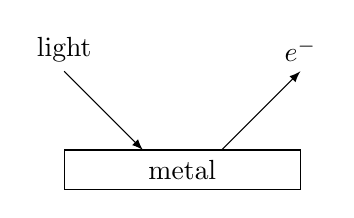
\begin{tikzpicture}
        \draw (0,0) rectangle node {metal} (3,0.5);
        \draw[-latex] (0,1.5) node[above] {light} -- (1,0.5);
        \draw[-latex] (2,0.5) -- (3,1.5) node[above] {$e^-$};
    \end{tikzpicture}
    \caption{光电效应图示}
\end{figure}
日文为光電効果,指金属在受到光的照射后释放出电子的现象,并特称这种电子为\underline{光电子},称产生的电流为\underline{光电流}。一般使用光电管作为实验装置。
\begin{figure}[ht!]
    \centering
    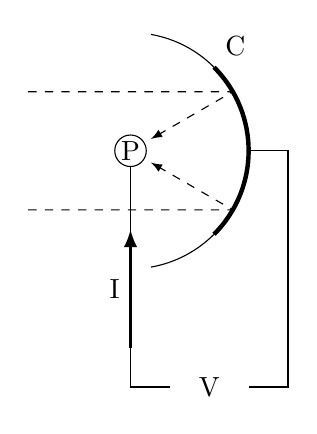
\begin{tikzpicture}
        \draw (0,0) -- (0,-3) -- (0.5,-3);
        \draw (1.5,0) -- (2,0) -- (2,-3) -- (1.5,-3);
        \node at (1,-3) {V};
        \draw[very thick,-latex] (0,-2.5) -- node[left] {I} (0,-1);
        \filldraw[draw=black,fill=white] (0,0) circle (0.2) node {P};
        \draw (80:1.5) arc (80:-80:1.5);
        \draw[ultra thick] (45:1.5) node[above right] {C} arc (45:-45:1.5);

        \draw[dashed, -latex] (150:1.5) -- (30:1.5) -- (30:0.3);
        \draw[dashed, -latex] (-150:1.5) -- (-30:1.5) -- (-30:0.3);
    \end{tikzpicture}
    \caption{光电管}
\end{figure}
这个现象为海因里希·赫兹(德国)于1887年首次发现,菲利普·莱纳德(德国)用实验验证了其重要规律,最后由爱因斯坦(美国)提出了正确的理论机制。
\begin{itembox}[l]{光电效应结论}
    \begin{itemize}
        \item 光电效应发生与否只取决于照射光的频率。
        \item 金属释放出的电子的动能仅依存于照射光的频率,与其强度无关。
        \item 增大照射光的光强会使得金属释放出的电子增多。
    \end{itemize}
\end{itembox}
也就是说当照射光的频率小于某个数值时无论光强如何大光电效应都不会发生;相反只要频率大于该值,无论光强如何小光电效应都会发生。一般称这个阈值$\nu_0$为\underline{极限频率},日文为限界振動数。然而以上的结论却与既有的理论不符。
\begin{itemize}
    \item 常理认为金属内的自由电子接收到来自于的光波的能量,从而离开金属,而且光波的能量同时依存于其频率和振幅。因此,即便频率很小但只要振幅足够,电子理应也能够得到足够的能量离开金属。这点却与结论一不符。
    \item 同理光强越强电子也应该得到更多的能量,这与结论二不符。
    \item 更令人意外的是虽然光强没有增加,每个电子的能量但却增加了电子的数量,这使得结论三变得不符合直觉。
\end{itemize}

\subsubsection{光量子假说}

为了合理解释光电效应的实验结果,爱因斯坦破天荒地提出了光量子假说,即光虽然是一种电磁波具有波动的性质(当时不争的事实),但同时也会表现出粒子的性质。
\begin{itembox}[l]{光量子假说}
    \begin{itemize}
        \item 光也是粒子,即光子。光强由光子数决定。
        \item 光子所携带的能量与其频率成比例,即$E=h\nu$($h$为普朗克常数)。
        \item 光子所携带的动量与其波长成反比,即$p=\frac{h}{\lambda}$
    \end{itemize}
\end{itembox}
基于以上的两个假设便可以解释一切光电效应的结论。
\begin{itemize}
    \item 光是粒子,一个光子给一个电子传递能量,光子越多(光强越大)便可以给予更多的电子能量,因此释放出的电子也会越多。
    \item 光子的能量取决于其频率,其自身能量越大能够给予电子的也就越多,然而光强只改变了光子的数量,因此电子的动能只和光子的频率有关。
\end{itemize}
至于结论一,我们先需要明确一下自由电子离开金属的具体细节。尽管电子可以在金属中自由移动,但其仍然会收到来自于金属阳离子的库仑力,并对其有一定的束缚作用。因此为了离开金属,就必须先克服掉这个束缚。将克服束缚所需的能量称为\underline{逸出功},日文为仕事関数\footnote{中文也有功函数的说法。}。
\begin{itemize}
    \item 若是光子所携带的能量足够电子克服金属的束缚,那么电子便可以离开金属。相反,当一个光子无法提供足够的能量,无论整体光强再大也无法使金属释放任何电子。
    \item 因此被释放出的电子的动能即为克服束缚后光子能量的剩余部分。
\end{itemize}

\subsubsection{光电效应理论解释}

将上一节的语言描述整理为数式即为
\begin{equation*}
    h\nu=W+K_{max}
\end{equation*}
其中$h\nu$为光子的能量,$W$为逸出功,$K_{max}$为电子的最大动能。
\begin{figure}[ht!]
    \centering
    \begin{tikzpicture}
        \draw[-latex] (-0.2,0) -- (2.5,0) node[right] {$\nu$};
        \draw[-latex] (0,-1.5) -- (0,1.5) node[above] {$K_{max}$};
        \draw[dashed] (0,-1) node[left] {$-W$} -- (1,0);
        \draw (1,0) node[below right] {$\nu_0$} -- (2,1);
    \end{tikzpicture}
    \caption{光电效应函数图}
\end{figure}
从图中可以发现纵截距的绝对值为逸出功,横截距为极限频率,斜率为普朗克常数。

此外,上式中的$K_{max}$可以通过调整实验装置的方式求得。当阳极P的电压高于阴极C的电压时,电子会逆着电场方向流向阳极,产生光电流。逐渐调低阳极电压直至低于阴极电压,此时电子为了来到阳极,需要不断消耗自身动能克服电场力的阻碍。最终若是某一阳极电压$V_0$下不再存在光电流,即证明动能最大的电子也无法到达,即可通过$K_{max}=eV_0$的方式求得电子的最大动能。一般称这个电压为\underline{遏制电压},日文为阻止電圧。

\subsection{X射线}

X射线一般可认为是波长短于紫外线的电磁波,由于发现之初并没能认清其本质,故命名为X射线。其发生机制为用高能电子轰击金属,撞击过程中电子减速,损失的动能以光子的形式释放,从而形成X射线。将收集到的X射线按照波长和其强度的关系绘制可得如下关系图。其中突出的部分称为固有X射线,剩下的部分称为连续X射线。
\begin{figure}[ht!]
    \centering
    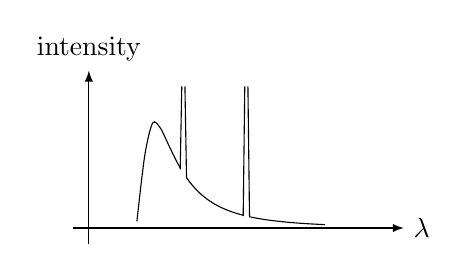
\begin{tikzpicture}[xscale=1]
        \draw[-latex] (-0.2,0) -- (4,0) node[right] {$\lambda$};
        \draw[-latex] (0,-0.2) -- (0,2) node[above] {intensity};

        \draw[domain=0.61:3] plot[smooth] (\x, {1/((\x-0.5)^3*exp(1/(\x-0.5))});
        \draw[color=white, line width=2pt] (1.2,0.1) -- (1.2,2);
        \draw[color=white, line width=2pt] (2,0.1) -- (2,2);

        \draw (1.16,0.75) -- (1.18,1.8); \draw (1.24,0.65) -- (1.22,1.8);
        \draw (1.96,0.15) -- (1.98,1.8); \draw (2.04,0.15) -- (2.02,1.8);
    \end{tikzpicture}
    \caption{X射线谱}
\end{figure}

\subsubsection{连续X射线}

当电子行进到金属的原子核附近时,会收到来自于原子核的引力而发生路径的偏转,在这个过程中电子丢失动能并转化为光子释放出去,从而形成了连续X射线。
\begin{itemize}
    \item 电子具有的初动能有上限,因此不会存在能量高于其初动能的X射线。
    \item 电子可以损失的能量连续,因此整体函数也是连续的。
\end{itemize}

\subsubsection{固有X射线}

当高能电子撞击到原子的核外电子使其发生跃迁时,会产生出能级跃迁所对应的能量的光子,这些时刻在图中的凸起处得以体现\footnote{本人编辑本文时未能找到解释固有射线强度高于连续射线强度的文章,在此根据个人理解简作说明。原子核所占空间远小于核外电子,因此核外电子好似内部原子核的屏障一般。如此一来高能电子会有更大的概率与核外电子相撞而产生固有射线,相反只有巧妙避开了核外电子的幸运儿才会在和原子核的作用下产生连续射线。所以按照光量子假说固有射线所对应的光子更多,即其强度就会更强。以上内容为个人解释,尚未有材料佐证,仅供参考以辅助理解。}。由于跃迁的能量取决于金属本身的原子结构,所以增大电子的加速电压虽然会使得图像整体左移,却不会改变凸起处的位置。

此外,X射线也是电磁波,和光一样也会表现出粒子性。其波动性可由布拉格反射验证,粒子性可由康普顿效应验证。

\subsection{物质波}

在上两节中,物理学家破天荒地为波引入了粒子性,从而合理解释了一些现象。在此基础上德布罗意(法国)认为既然波可以有粒子性,那么粒子同样也可以具有波动性,因而提出了物质波的概念。
\begin{equation*}
    \lambda=\frac{h}{mv}
\end{equation*}
而后的实验也证明了德布罗意的猜想,证实了物质的波粒二象性。比如我们可通过定义式求出由电压$V$加速后电子的物质波长。
\begin{equation*}
    eV=\frac12mv^2\to
    \lambda=\frac{h}{\sqrt{2meV}}
\end{equation*}
